%
% polygon.tex
%
% (c) 2020 Prof Dr Andreas Müller, Hochschule Rapperswil
%
\section{Lineare Interpolation und Polygonzüge
\label{buch:section:lineareinterpolation}}
Oft sind von einer Funktion nur einzelne Werte bekannt, doch meist reicht
dies, den ungefähren Verlauf ihres Graphen zu erahnen.
Unter der Annahme, dass sich die Funktion zwischen den bekannten Werten
nicht zu ``wild'' verhält, können Werte zwischen den bekannten Werten
abgeschätzt werden.
In diesem Abschnitt soll daher die folgende Aufgabe gelöst werden.

\begin{aufgabe}
\label{buch:aufgabe:basicinterpolation}
Gegeben $n+1$ sogenannte {\em Stützstellen}
\index{Stützstelle}%
\[
a=x_0<x_1<x_2<\cdots<x_{n-1}<x_n=b
\]
im Intervall $[a,b]$ und bekannte Funktionswerte $f_i$, $0\le i\le n$,
finde eine stetige Funktion $f\colon[a,b]\to \mathbb R$ derart, dass
$f(x_j)=f_j$ für $0\le j\le n$.
\end{aufgabe}

\subsection{Lineare Interpolation
\label{buch:subsection:lineareinterpolation}}
Die Aufgabe~\eqref{buch:aufgabe:basicinterpolation} ist zu wenig präzise
gestellt, es gibt unendlich viele Lösungen.
\index{lineare Interpolation}%
\index{Interpolation!linear}%
Es müssen daher zusätzliche Bedingungen an die gesuchte Funktion $f$
gestellt werden, damit die Lösung eindeutig bestimmt wird.
Ein mögliche solche Bedingung ist, dass die Funktion $f$ in jedem
Teilintervall zwischen aufeinanderfolgenden Stützstellen linear ist.
In diesem Fall haben die Werte ausserhalb des Intervalls offenbar 
keinen Einfluss auf den Verlauf im Inneren des Intervalls, es genügt
also das Problem mit nur zwei Stützstellen zu lösen.

\begin{satz}
\label{buch:satz:lineareinterpolation}
Die einzige auf dem Intervall $[x_i,x_{i+1}]$ definierte lineare Funktion 
\index{lineare Funktion}%
\index{Funktion!linear}%
$f(x)$ mit Funktionswerten $f(x_i)=f_i$ und $f(x_{i+1}) = f_{i+1}$
hat im Punkt $x\in[x_i,x_{i+1}]$
den Wert
\begin{equation}
f(x)
=
\frac{f_{i+1}-f_i}{x_{i+1}-x_i} (x-x_i) + f_i
=
\frac{x-x_{i+1}}{x_i-x_{i+1}} f_i
+
\frac{x_{i}-x}{x_i-x_{i+1}} f_{i+1}
=
f_il_i(x) + f_{i+1}l_{i+1}(x)
\label{buch:eqn:lineareinterpolation}
\end{equation}
mit den linearen Funktionen
\begin{equation}
l_i(x) = \frac{x-x_{i+1}}{x_i-x_{i+1}}
\qquad\text{und}\qquad
l_{i+1}(x) = \frac{x_i-x}{x_i-x_{i+1}}.
\label{buch:eqn:linl0l1}
\end{equation}
\end{satz}

\begin{proof}[Beweis von Satz~\ref{buch:satz:lineareinterpolation}]
Die beiden linearen Funktion $l_i(x)$ und $l_{i+1}(x)$ haben an den 
Intervallenden die speziellen Werte
\[
\begin{aligned}
l_i(x_i)&=1  &\qquad&\qquad& l_{i+1}(x_i)&=0 \\
l_i(x_i)&=0  &\qquad&\qquad& l_{i+1}(x_i)&=1,
\end{aligned}
\]
wie man durch Einsetzen unmittelbar bestätigen kann.
Die zweite Form in~\eqref{buch:eqn:lineareinterpolation}
ist daher als Linearkombination
\[
f(x)=f_il_i(x) + f_{i+1}l_{i+1}(x)
\]
linearer Funktionen wieder
linear, und dank der speziellen Werte von $l_i$ und $l_{i+1}$ folgt
unmittelbar, dass
\begin{align*}
f(x_i)&=f_il_i(x_i) + f_{i+1}l_{i+1}(x_i) = f_i\cdot 1 + f_{i+1}\cdot 0= f_i\\
f(x_{i+1})&=f_il_i(x_{i+1}) + f_{i+1}l_{i+1}(x_{i+1})= f_i\cdot 0 + f_{i+1}\cdot 1=f_{i+1}
\end{align*}
gilt.

Der Bruch
\index{Bruch}%
\[
m = \frac{f_{i+1}-f_i}{x_{i+1}-x_i}
\]
ist die Steigung der Geraden durch die Punkte $(x_i,f_i)$ und
$x_{i+1},f_{i+1})$.
\index{Steigung}%
Der erste Ausdruck auf der rechten Seite in
\eqref{buch:eqn:lineareinterpolation} ist
also $f(x)=m(x-x_i)+f_i$, dies ist die Gleichung einer Geraden
mit Steigung $m$ durch den Punkt $(x_i,f_i)$, sie verläuft natürlich
auch durch den Punkt $(x_{i+1},f_{i+1})$.
\index{Gerade}%
\end{proof}


\subsection{Polygonzüge
\label{buch:subsection:polygonzuege}}
\begin{figure}
\centering
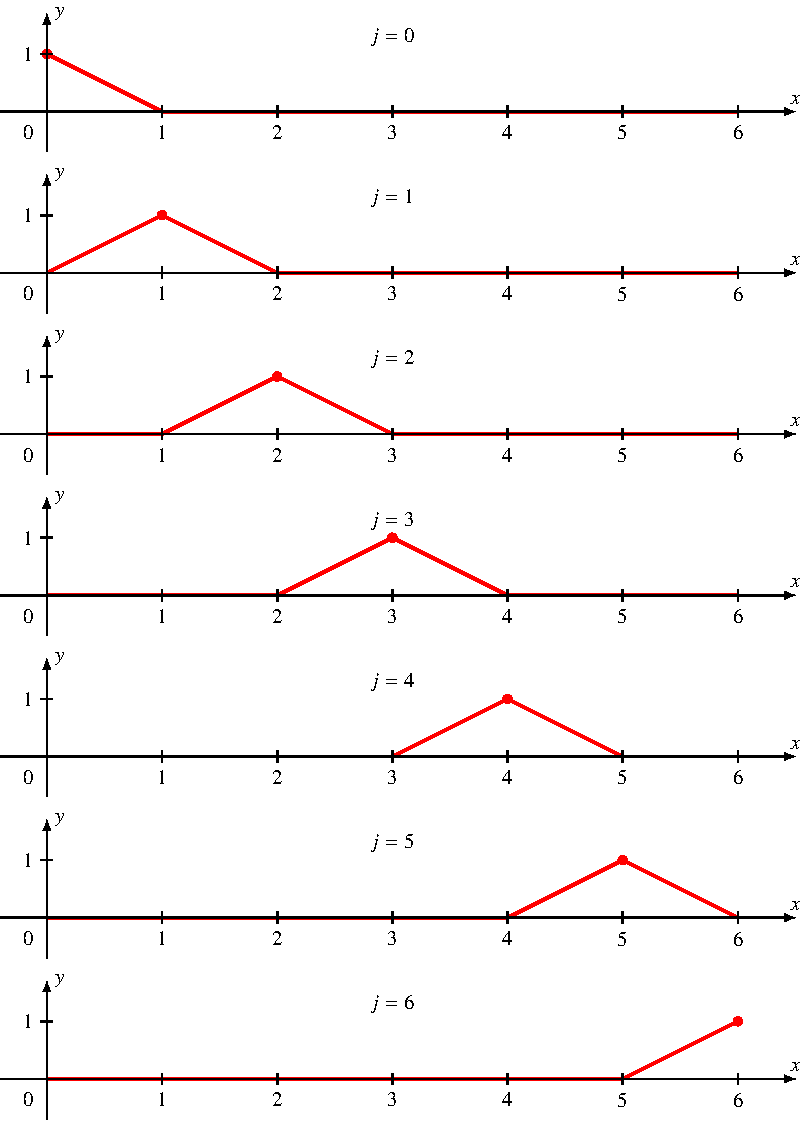
\includegraphics{chapters/30-interpolation/figures/polygon.pdf}
\caption{Basisfunktionen für die lineare Interpolation einer 
Funktion $f\colon[0,6]\to\mathbb R$ mit Stützstellen $0,1,\dots,6$
\label{buch:figure:polygonbasis}}
\end{figure}
\eqref{buch:eqn:linl0l1}
Wendet man das Resultate von Satz~\ref{buch:satz:lineareinterpolation}
auf jedes Teilintervall an, entsteht eine Interpolationsfunktion, deren
Graph ein Polygonzug ist.
\index{Interpolationsfunktion}%
\index{Graph}%
\index{Polygonzug}%
Eine solche Funktion lässt sich einfacher beschreiben mit Hilfe
der Interpolationsfunktionen mit den speziellen Werten
\begin{equation}
l_i(x_j) = \delta_{ij} =\begin{cases}
1&\qquad i=j\\
0&\qquad\text{sonst.}
\end{cases}
\label{buch:eqn:interpolation:basis}
\end{equation}
Die Funktionen sind in Abbildung~\ref{buch:figure:polygonbasis} für
die Stütztstellen $x_0=0$, $x_1=1$, \dots , $x_6=6$ dargestellt.
Die lineare Interpolationsfunktion kann jetzt als Linearkombination
der Funktionen $l_i$ geschrieben werden:
\begin{equation}
f(x)
=
\sum_{j=0}^n f_j l_j(x).
\label{buch:eqn:interpolation:linearkombination}
\end{equation}
Diese Lösung des Interpolationsproblems kann für alle weiteren
Interpolationsansätze in diesem Kapitel als Vorlage dienen.
Es geht nämlich nicht darum, eine Interpolationsfunktion in
geschlossener Form hinzuschreiben, dies ist für die Funktionen $l_j(x)$
ohnehin nicht möglich.
Es ist nur nötig, dass Funktionswerte $f(x)$ effizient berechnet
werden können.
Die letztere Aufgabe ist gelöst, wenn man die Funktionen $l_j(x)$
effizient berechnen kann.
Es ist dann nur noch die
Linearkombination~\eqref{buch:eqn:interpolation:linearkombination}
zu bilden.

Die Wahl der Funktionen $l_j(x)$, die natürlich die Bedingungen
\eqref{buch:eqn:interpolation:basis} erfüllen müssen,
bestimmt die Eigenschaften der
Interpolationsfunktion, die nach 
\eqref{buch:eqn:interpolation:linearkombination}
gebildet wird.
In diesem Abschnitt waren die $l_j$ stückweise lineare Funktionen,
also auch die Funktion $f(x)$.
\index{stückweise linear}%
Im nächsten Abschnitt sollen die Funktionen Polynome sein,
also wird die Interpolationsfunktion ebenfalls ein Polynom sein.






